% The chapters for hmi/animation, for inclusion within a master LaTeX document
% include files must specify a path like \hmianimationreportdir/filename
% where \hmianimationreportdir should be defined in the master document.
% We have a fall back:
\ifx \hmianimationreportdir \undefinedmacro \def \hmianimationreportdir{.} \fi
\ifx \webserver \undefinedmacro \def \webserver{http://elckerlyc.sourceforge.net/javadoc/Hmi/} \fi

\chapter{The HmiAnimation package}
The hmi/animation package is meant for 3D animation purposes.

\section{Overview}

The hmi.animation package defines classes for animation of objects and humanoids inside
a virtual environment. It deals only with abstract descriptions of such environments,
but not, for instance, the implementation of visualization virtual environments.
As a consequence, it is necessary to combine this package either with
simple 2D graphics, or with more complicated 3D graphics.
The basic entity defines in this package is the VObject. (``Virtual and/or Visual Object'').
Such VObjects have a defined name, they define some set of \emph{attributes} and they define a
limited set of physical attributes, like position and orientation in 3D space.
Moreover, VObjects are arranged in a hierarchical scene-graph like arrangement,
where VObjects are built up from smaller parts.
There can be a direct \emph{parent-child relationship} between two VObjects, or some
VObject V can be considered a \emph{part} of some other VObject P if it is \emph{recursively}
a child of P.
This scene-graph takes into account the positioning and orientation (and possibly scaling) of child parts, relative
to the position and orientation of their parent VObject.
The relative position, called the \emph{translation}, the relative \emph{orientation}, and the relative \emph{scaling} together define the \emph{local transform} of a VObject.

See the \href{\webserver}{javadoc}.

%A VirtualObject has a
%unique identity, called its ``Id'', and if you want, than that's all there is to it.
%In practice, virtual objects have some more structure:
%\begin{itemize}
%\item They can define \emph{attributes}
%\item They can define a \emph{Category}, to be understood
%as a category or class as defined by ontologies. (Since the word ``class'' is heavily overloaded,
%and has a conflicting meaning already for Java programs, we use ``category'', like in %\ref{}%)
%\item They can have \emph{child elements}, which are VirtualObjects themselves.
%\end{itemize}
%
%VirtualObject is a base class, to be extended by other classes. A first step here is the VisualObject class,
%which extends VirtualObject, and adds a number of properties like physical location and possibly orientation
%in 3D space. VisualObjects can also act as the ``target'' of various animation techniques,
%which modify location or orientation. Since VisualObjects are VirtualObject, they can have parts that
%are VisualObjects themselves. There are VisualObjectInterpolators that are able to control
%the orientation (and location) of all parts of a structured VisualObject in an interpolation process,
%based on key framing. This forms the basis for, for instance, avatar animation, where avatars posses
%a certain ``bone structure''.
%
%The name ``visual'' object is not completely appropriate, since no visualization
%is actually \emph{required} for VisualObjects.
%Instead, a VisualObject acts as a common ground for potentially maby forms of visualization,
%in 3D or 2D, possibly at the same time.
%All such visualizations need location and orientation information, regardless of whether they are 2D or 3D,
%and regardless of the rendering technique being used.
%The actual visualizations are defined outside the environment package, as they
%are tightly bound to some particular rendering technique.
%As a result, the environment package is independent of for instance the Java3D based parlevink.x3d package.
%A small concession here is that as far as the usage of positions an orientations is concerned,
%we rely on the javax.vecmath package. This package is usually distributed as part of the java3D packages, but it is
%available as a separate jar file.



\section{XML encoding of VObjects}

%The VirtualObjectAdapter class is itself an extension of XMLStructureAdapter,
%so a lot of useful techniques and methods are available for all extensions of VirtualObjectAdapter and
%VisualObjectAdapter.
%(See also the documentation for XMLStructureAdapter in the parlevink.xml package)
%Although it would be possible to re implement basic XMLStructure methods ``from the ground up'' so to say,
%this is in general not a good idea. In such cases, you would need to take care of generic VirtualObject/VisualObjectAdapter data.
%Rather than doing this, it is better to re implement a few selected VirtualObjectAdapter methods, which will
%ensure that all such ``generic'' data is taken care of.
%The layout VirtualObjectAdapter encodings is like the following: (not all parts need be present)
%\begin{verbatim}
%<VirtualObjectAdapter (VirtualObject  XML attributes) >
%   <Attributes>
%   ...(encoded VirtualObject attributes)
%   </Attributes>
%   <Children>
%   ... (encoded VirtualObject parts)
%   </Children>
%</VirtualObjectAdapter>
%\end{verbatim}
%We remark that when the virtual object defines no attributes at all, then
%the \verb"<Attributes>..</Attributes>" section
%is omitted. Also, when there are no child parts at all, the \verb"<Children> ...</Children>"
%section will be omitted.
%Why did we say that the encoding is ``like the following''?
%Because all of it can be modified for classes that derive
%from VirtualObjectAdapter.
%For instance, the  names of the tags can be chosen differently, and the \verb"<Children>" tag could even be
%omitted altogether.
%As a starter: the XML tag (``VirtualObjectAdapter'') is not really appropriate for any derived class,
%and should be replaced by an better tag name, preferably some that mimics the class name.
% Say you have a class called ``project.Vproject.MyVObject'', then the preferred tag would be ``MyVObject''.
%This is done as usual for all XMLStructureAdapters:
%by redefining the public String getXMLTag() method, which the tag name for that class, and  which would
%be the String ``MyVObject'' in the example above.
%It is also highly desirable to register this tag name with the parlevink.xml.XML class, in order to
%enable automatic reconstruction of objects from XML code. (See the parlevink.xml documentation)
%The next step is that the derived class might need to add its own XML attributes to the
%start tag (i.e. within the \verb"<MyVObject ......>") section.
%The appropriate way to do this is to (re)implement the \verb"appendAttributeString" method.
%This method should start with calling \verb"super.appendAttributeString(..)", which will take care
%of all attributes contributed by parent classes. We give a small sample of this type of code:
%\begin{verbatim}
%public StringBuffer appendAttributeString(StringBuffer buf) {
%   super.appendAttributeString(buf);
%   appendAttribute(buf, "myAttribute1", attr1.x, attr1.y);
%   if (attr2 != null) appendAttribute(buf, "attr2", attr2);
%      appendAttribute(buf, "scale", sx, sy, sz);
%   return buf;
%}
%\end{verbatim}
%Here we have assumed that we want to add two attributes, called ``attr1'' and attr2''.
%The first one has two fields, both of which are floats, and the second attribute has a (single) String
%typed value. In general, you must append to the ``buf'' StringBuffer, but in many cases you
%can use the appendAttribute method, defined in XMLStructureAdapter. (This method allows all kinds
%of arguments, and will encode them, see the parlevink.xml documentation)
%
%The counterpart of this is of course, how to \emph{decode} attributes.
%A similar strategy like the one for encoding is available: reimplement the \verb"decodeAttribute" method, and for all attributes that
%you don't recognize, call super.decodeAttribute().
%The boolean value that is returned denotes whether the attribute name was recognized. An example:
%\begin{verbatim}
%public boolean decodeAttribute(String attrName, String valCode) {
%   if (attrName.equals("attr1")) {
%      float[] t = XMLStructureAdapter.decodeFloatArray(valCode, null);
%      setAttr1(t);
%      return true;
%   } else if (attrName.equals("attr2")) {
%      attr2 = valCode
%      return true;
%   } else {
%      return super.decodeAttribute(attrName, valCode);
%   }
%}
%\end{verbatim}
%decodeAttribute will be called for each separate attribute in turn;
%it checks for the attribute name, and if it is recognized
%the String typed attribute value must be decoded. In general that would involve converting
%the ``valCode'' String to the appropriate data type.
%Note that XMLStructureAdapter includes a few methods that take care of annoying problems like
%dealing with sequences of numbers. (For example, if the attribute would look like \verb/attr1="11.1 33.3"/,
%then decodeAttribute will be called with the Strings ``\verb/attr1/.'' and ``\verb/11.1 33.3/''.
%The decodeFloatArray would turn the latter String into a Float array \verb"t" with two elements, and the
%\verb"setAttr1(t)" in the example above is supposed to set the value of the attribute, using such an array value.
%
%The next modification you would like to make to the generic VirtualObjectAdapter layout is
%to add what is called ``contents'', or ``PCDATA'' in XML terminology.
%This is the section between the \verb"<MyVObject>" tag and the \verb"</MyVObject>" tag.
%The default is to include the encoding of the VirtualObject attributes (not to be confused with the
%XML style attributes \emph{within} the \verb"<MyVObject...>" tag), followed
%by the encoding of child parts.
%The code fragments responsible for this are the following:
%\begin{verbatim}
%public StringBuffer appendContent(StringBuffer buf, int tab) {
%   appendVOContent(buf, tab+TAB);
%   appendChildren(buf, tab+TAB);
%   return buf;
%}
%
%public StringBuffer appendVOContent(StringBuffer buf, int tab) {
%   if (attributes != null) {
%      buf.append('\n');
%      attributes.appendXML(buf, tab);
%   }
%  return buf;
%}
%\end{verbatim}
%From this the reimplementation strategy follows:
%\begin{itemize}
%\item If you want to add some ``content'', in the form of XML elements, \emph{after} the VirtualObjectAdapter
%Attribute section, but \emph{before} the children section, then re implement just the \verb"appendVOContent" method, like for example:
%\begin{verbatim}
%public StringBuffer appendVOContent(StringBuffer buf, int tab) {
%   super.appendVOContent(buf, tab)
%   // add MyVObject content
%   return buf;
%}
%\end{verbatim}
%\item If you want to reorder the content more drastically, you will have to re implement the
%\verb"appendContent" method.
%\end{itemize}
%
%Finally, we must discuss how this extra content is to be \emph{decoded}.
%Again, you should re implement the appropriate VirtualObjectAdapter method,
%which in this case is the \verb"decodeXMLElement" method.
%To understand the role of this method within the decoding process, we provide the
%\verb"decodeContent" and the \verb"decodeXMLElement" methods from VirtualObjectAdapter
%itself:
%
%\begin{verbatim}
%public void decodeContent(XMLTokenizer tokenizer) throws IOException {
%   while (tokenizer.atSTag()) {
%      boolean decoded = decodeXMLElement(tokenizer, tokenizer.getTagName());
%   }
%}
%
%public boolean decodeXMLElement(XMLTokenizer tokenizer, String stag)
%throws IOException {
%   if (stag.equals(attributesTag)) {
%      allocate();
%      attributes.readXML(tokenizer);
%      return true;
%   } else if (stag.equals(childrenTag)) {
%      tokenizer.takeSTag();
%      while (tokenizer.atSTag()) {
%         addChild((VirtualObjectAdapter) XML.createXMLStructure(tokenizer));
%      }
%      tokenizer.takeETag(childrenTag);
%      return true;
%   } else {
%      Console.println("Skipping unknown VirtualObject tag: " + stag);
%      tokenizer.skipTag();
%      return false;
%   }
%}
%\end{verbatim}
%
%These code fragments suggest how to re implement the \verb"decodeXMLElement" method:
%The code should be like the following:
%\begin{verbatim}
%public boolean decodeXMLElement(XMLTokenizer tokenizer, String stag)
%throws IOException {
%   if (stag.equals(MyContentTag1)) {
%      // process content element type 1
%      return true;
%   } else if (stag.equals(MyContentTag2)) {
%      // process content element type 2
%      return true;
%   } else {
%      return super.decodeXMLElement(tokenizer, stag);
%   }
%}
%\end{verbatim}
%
%The VirtualObject base class assumes that the \verb"<Children>" tag
%is used to include a number of child VirtualObject elements.
%This tag can be renamed, or it can be omitted.
%This can be done by re implementing the \verb"getChildrenTag()" method.
%The default VirtualObject implementation returns the String \verb"Children".
%If the method returns null, the encoding will omit the Children tag.
%Note that extensions of VirtualObject or VisualObject can introduce any sort of elements
%outside any ``Children'' section, including elements that should be regarded as child elements.
%It is important that such elements are included as ``child'' by calling the
%addChild(VirtualObject) method from the VirtualObjectAdapter superclass.
%\begin{verbatim}
%   public String getChildrenTag() {
%      return CHILDRENTAG;
%   }
%\end{verbatim}
%
%
%\section{Visualization}
%
%Although VisualObjects appear to be ``visual'' objects, this is only partly true.
%It is more appropriate to think of VisualObjects as VirtualObjects that have one (and possibly more)
%visualization attached to it. The dominant visualization technique at this point in time is based on
%Java3D/X3D techniques. An alternative, as yet not fully implemented, is a Java2D visualization technique.
%VisualObjects do have a number of attributes and properties that are shared among
%all visualizations: they possess a position and an orientation in (3D) space.
%Because of the hierarchical structure of VisualObjects, the position and orientation are really
%\emph{relative} to the position and orientation of some parent VisualObject, and for
%this reason these attributes are called \emph{translation}, rather than position, and
%\emph{rotation}, rather than  orientation. (This terminology stems directly from Java3D, VRML, and X3D)
%The coupling between a VisualObject and its visualization(s) has two aspects: the programming
%API, and the XML/X3D encoding aspect.
%To start with the latter: this is rather easy. The XML encoding of VisualObjects allows
%XML content to be (children) VisualObjects, as well as Visualizations.
%The latter are regarded as the Visualization that belongs to that VisualObject.
%For instance, consider the following example:
%\begin{verbatim}
%   <VisualObject id = "box1"
%     translation = "-1.2 0.5 0.0" rotation = "1 0 0 0.4">
%         <Shape>
%            <Appearance DEF = "app1">
%                  <Material DEF="m1" diffuseColor="1.0 0.0 0.1">
%                  </Material>
%            </Appearance>
%            <Box size="1.0 0.3 1.0" DEF="box1">
%            </Box>
%         </Shape>
%   </VisualObject>
%\end{verbatim}
%This defines a VisualObject ``box1'', without any VisualObject parts. It does have a
%3D visualization though, in the form of an X3D Shape.
%A more complicated example:
%\begin{verbatim}
%<VisualObject id = "hammer" translation = "0.0 -0.5 0.0">
%   <VisualObject id = "cyl" translation = "1.2 0.5 0.0"
%                    rotation = "1 0 0 0.7" dynamic="true">
%      <VisualObject id = "box2"
%         translation = "0.0 1.0 0.0" dynamic = "true">
%            <Shape>
%               <Appearance >
%                  <Material diffuseColor="0.0 1.0 1.0" />
%               </Appearance>
%               <Box size = "0.4 0.4 0.6"/>
%            </Shape>
%      </VisualObject>
%      <Shape>
%        <Appearance >
%           <Material USE="m1"/>
%           <ImageTexture url="x3d/gelemuur.jpg" />
%        </Appearance>
%        <Cylinder height="1.5" radius = "0.2"/>
%      </Shape>
%  </VisualObject>
%</VisualObject>
%\end{verbatim}
%This defines a VisualObject ``hammer'' with a part called ``cylinder'', which has an X3D Shape
%visualization. (The cylinder shape, with the ``gelemuur.jpg'' texture.
%The cylinder VisualObject has itself a child VisualObject, called ``box2''.
%The latter also has a visualization, in the form of an X3D box Shape.
%Both the cylinder and the box2 object are ``dynamic'', which indicates that they can be animated.
%In this case, the cylinder could rotate, and the box2 object could rotate on top of the cylinder.
%This pattern is also found in X3D/HAnim bone structures.
%
%The programming interface is slightly more complicated.
%Because visualizations can be either 3D or 2D, and because Java3D is not hard wired into
%the environment package, including the VisualObject class, the coupling between a VisualObject
%and its visualization(s) is established via two interfaces, defined within the environment package:
%VisualGroup and Visualization.
%A complication here is that the granularity, or level of detail at the VisualObject level
%and the visualization level need not be the same. A typical situation could
%be a ``shallow'' hierarchy at the VisualObject level, worked out only as far as is necessary
%for reasoning within object ontologies, combined with a highly detailed
%X3D visualization. The reverse is also possible: it is allowed to introduce VisualObjects
%that have no visualization at all levels of detail for both 2D and 3D visualizations.
%Think for instance of a ``book'' with many pages of text that are modeled at the VisualObject level
%as well as the 2D visualization level, but where only the book as a whole is modeled at the 3D visualization
%level.
%
%A VisualGroup is the counterpart of the VisualObject that is capable of building hierarchical ``scene graphs''.
%That is, a VisualGroup has methods addVisualChild and removeVisualChild, for adding and deleting children,
%of type VisualGroup. In addition, there are methods for setting the configuration
%( i.e. the translation, rotation, and scale) of an VisualGroup, and a few other attributes.
%It also defines a getType() method, which is used to classify the type of visualization.
%A Visualization is somewhat simpler: is has a getType() method like VisualGroup, and
%it has a method getVisualGroup() that will encapsulate the Visualization within a VisualGroup object.
%A Visualization is primarily used for the visualization of some VisualObject without parts.
%A second use is to visualize some VisualObject that does have parts at the VisualObject level,
%but where there is no need for any visualization of those parts, or at least there is no need
%for any explicit coupling between the VisualObject hierarchy and the visualization
%hierarchy. A typical case could be the ``book'' example introduced above.




\section{Interpolators}
%VisualObjects are object with a defined \emph{translation},i.e its 3D ``position'', and a \emph{rotation}
%, i.e. its ``3D orientation''. (Note we use ``translation'' and ``rotation'' as this is the
%common terminology used by  VRML, X3D, and Java3D.)
%Sometimes the 3D information might be visualized in 2D form, or might not be visualized at all,
%but conceptually everything takes place in 3D space. Therefore a translation is always a 3D vector,
%whereas a rotation is determined by a 4-tuple, either in the form of a quaternion, or else in the form
%of an axis of rotation and a rotation angle, a so called ``AxisAngle''.
%Optionally, one can define scale factors in addition to translation and rotation, but at this moment
%this is not fully integrated.
%VisualObjects can be combined in the form of hierarchical structures, via
%the parent-child relationship, inherited from the VirtualObject interface.
%A given node in this hierarchy can be seen as a root node, that has ``offspring'', in the form
%of children, children of children etc.
%The translations and rotations from a root node to one of its offspring nodes can be combined
%into resulting translation and rotation, the so called ``pathTranslation'' and ``pathRotation''.
%(Note: this works also when \emph{uniform} scaling is used, but it works no longer
%for non-uniform scaling)
%It is possible to set the translations and rotations along the
%VisualObject nodes along a path, and then to obtain the resulting pathTranslation and pathRotation.
%It is also possible to set the translation and rotation of a child node \emph{indirectly}, by
%specifying the desired pathTranslation and pathRotation of that child node.
%In general, translations and rotations (and sometimes also scaling) are specified at the same time.
%In such cases, it is sometimes easier to work with so called Configurations.
%There is a class \verb"Config3D" which is in essence a wrapper for a translation and a rotation.
%The VisualObjectAdapter class has setConfiguration methods that accept either
%a Config3D Object, or a translation and a rotation (and optionally a uniform scaling).
%
%\emph{Interpolation} is going one step further than just setting translations and rotations.
%In essence an \emph{interpolator} is a mapping from time stamps to interpolated values,
%that can be used as the basis for an animation, for instance.
%VRML/X3D/Java3D have a rather limited idea of interpolators: each interpolator controls
%one transform(group). This is also possible with VisualObjects, which can be seen as equivalent
%to the X3D/Java3D transform(group)s, as far as animation possibilities are concerned
%However, many VisualObjects have a more complicated, hierarchical structure.
%An example is the bone structure of an avatar, which can be seen as a structured VisualObject, where
%each joint in the bone structure corresponds to one (recursive) child element of the VisualObjet
%that describes the bone structure as a whole.
%In this case, the translation and rotation of the top level VisualObject describe the
%position and orientation of the avatar as a whole, within the virtual environment, whereas
%the rotations of the joints would describe the orientation of the body segments.
%In such cases, one needs an interpolator that controls many VisualObject(parts) at the same time.
%The basic (minimal) interface for interpolators is \verb"VisualObjectInterpolator".
%A VisualObjectInterpolator must have a defined start time, a defined ``target'' VisualObject, and
%methods for time interpolation.






\chapter{Animation, Physic simulation, and 3D rendering}



\section{Scenegraphs and Physics}

Animation is usually based upon VJoints, arranged into tree shaped scenegraphs.
This provided the interface between, on the one hand, rendering systems like those
from the hmi/graphics packages and, on the other hand, animation systems based upon interpolators, procedural animation,
or physics based simulation.

 Our animation structure is such that it supports splitting the rendering and animating processes into two separate threads. To allow this (and in the future possibly to allow multiple remote visualizations of the animation process running on a server), we separate the rendering and animation VJoint scene graphs (see Figure \ref{figuresg}). The local transform of the nodes under animation root is coupled to the render scene at its initialization. This coupling is many-to-one: one or more animation VJoints can steer a single render node. For example: a render node containing a deformable mesh for a humanoid is steered by a tree of animation VJoints representing the skeleton that steers the mesh. The animation tree is coupled to the render tree using the VJoint rotation/translation buffers: setting the rotation or translation of a animation tree VJoint directly sets the rotation in the corresponding render node. If animation and rendering occurs in different threads, access to the animation tree should be synchronized. This prevents the render thread reading partial information from the animation scene while it is still being updated by the animation thread. Typically the animation processes use copies of parts of the animation tree locally in time consuming animation processes and then uses a synchronized copy action to copy the resulting VJoint transformations to the animation scene. The render thread uses a synchronized action to calculate the global render node transformations from rotations in the animation tree (see also Figure \ref{threads}).

For a typical linking scenario see this \href{\hmianimationreportdir/typical_scenegraph.pdf}{scenegraph linking example}

\subsection{Example: animation algorithm in Elckerlyc}
The AnimationPlayerManager manages the animation proces in Elckerlyc. It contains an AnimationPlayer for each animated virtual human. It uses 3 copies of the joint tree of this humanoid: cur, prev, next, representing the joint rotations at $t$, $t-1$ and $t+h$ respectively. vjAni represents the root VJoint of the human in the animation joint tree. Animation is executed as follows:
\begin{enumerate}
\item run all animation players, in each animation player:
\begin{enumerate}
\item copy cur to prev, next to cur
\item run all procedural animations on next 
\item using prev, next and cur, calculate and apply the forces and torques generated by the kinematic motion to the human's physical body
\end{enumerate}
\item do a physics step
\item copy the physical body rotations to cur
\item copy the rotations of curr and its children to vjAni (and its children)
\end{enumerate}

\subsection{Synchronisation}
Acces to the VJoints in the Animation root should be synchronized to the animation sync:
\begin{verbatim}
synchronized(AnimationSync.getSync())
{
	do something with VJoints in animation root
}
\end{verbatim}
Access to objects controlled by physical simulation should be synchronized to the physics sync:
\begin{verbatim}
synchronized(PhysicsSync.getSync())
{
	access physical objects
}
\end{verbatim}

\begin{figure}
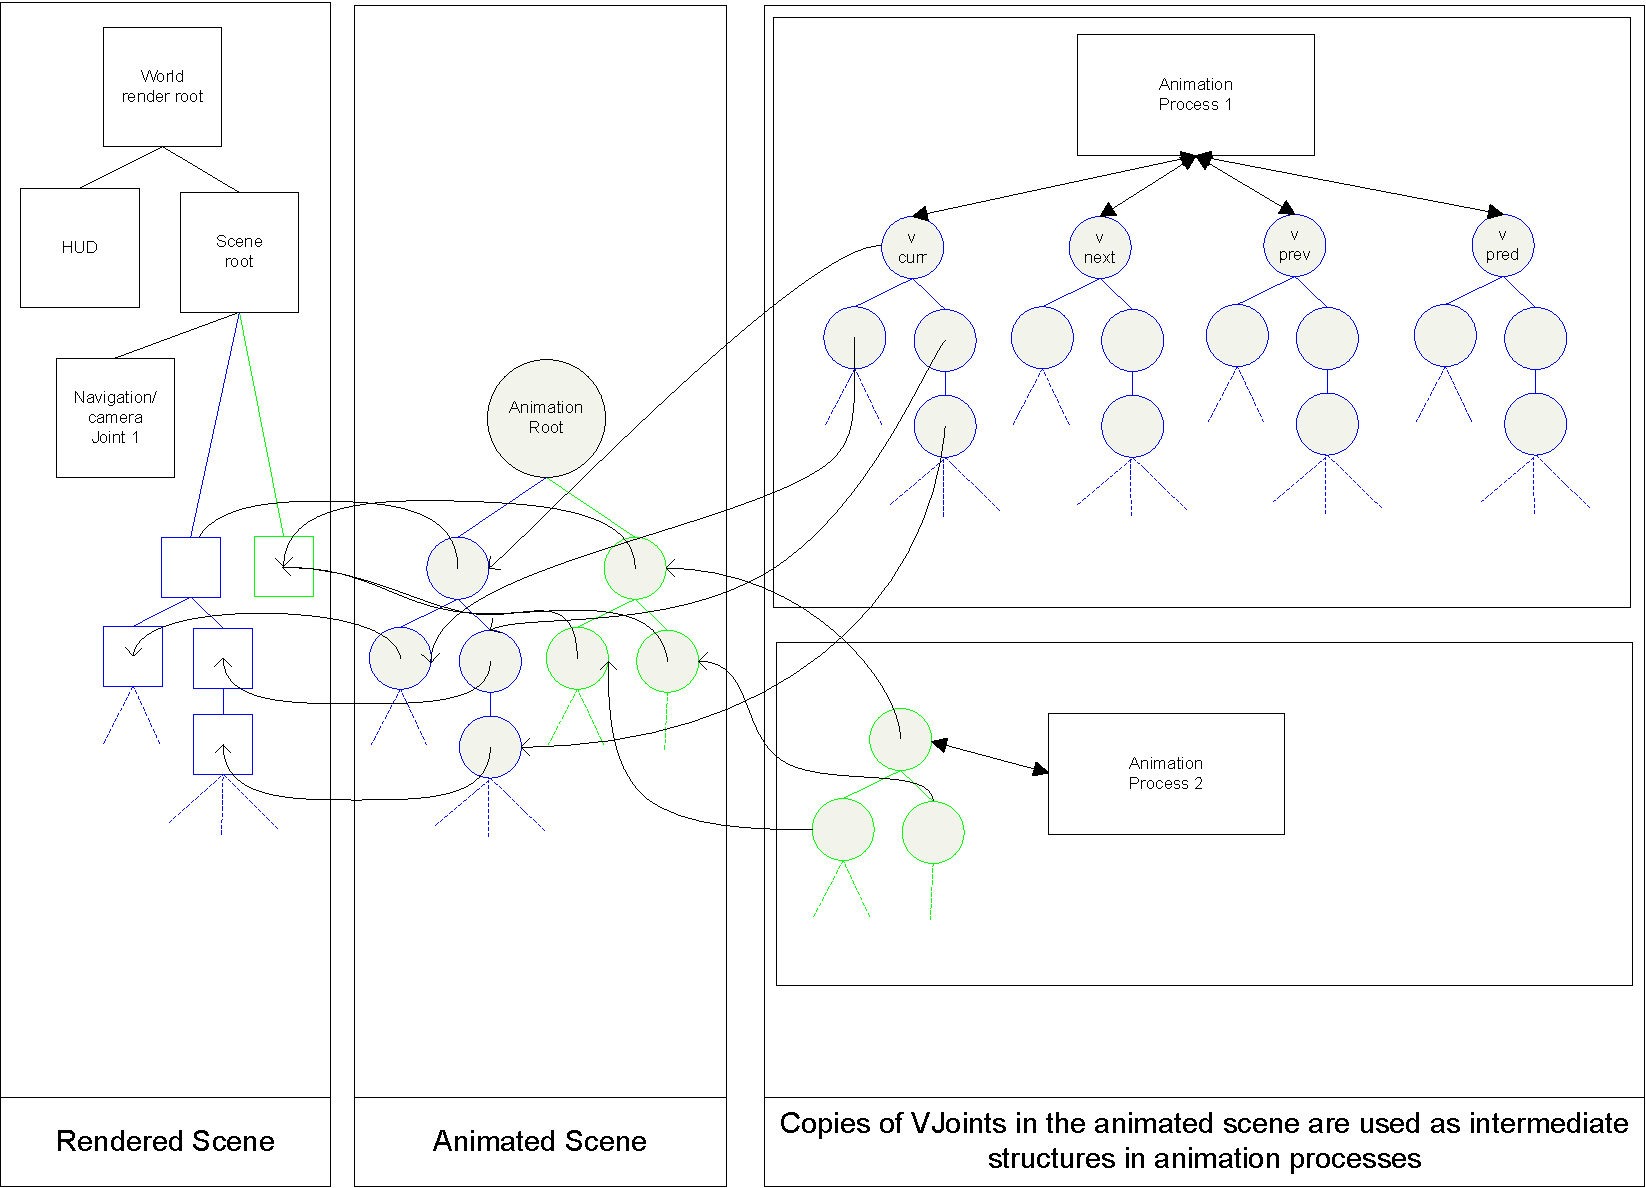
\includegraphics[width=13cm]{\hmianimationreportdir/typical_scenegraph}
\caption{\label{figuresg}Typical scenegraph layout}
\end{figure}

\begin{figure}
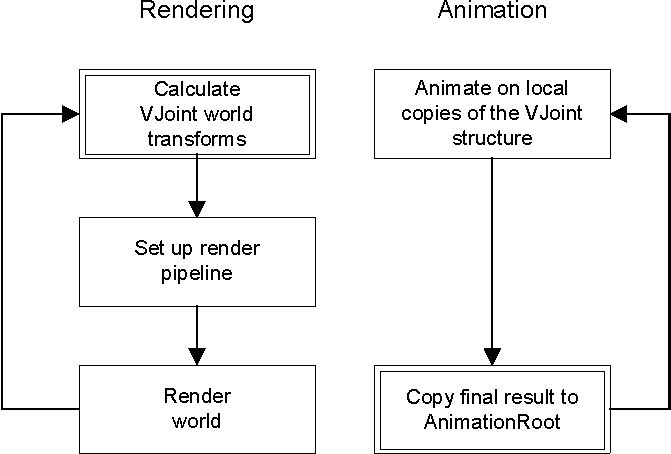
\includegraphics{\hmianimationreportdir/threads-crop}
\caption{\label{threads}Animation and rendering loops running in different threads. The processes with double lines are synchronized to each other.}
\end{figure}


 
\section{Procedural Animation}

\subsection{XML format}
...\\
Note that some symbols need to be XML encoded: $>$ as \&gt; , $<$ as \&lt; , \&\& as \&amp;\&amp; etc.
\subsubsection{JEP examples and custom macros}
Function of time ($0 \leq t \leq 1$) and float parameters (as constructed using \textless Parameter\textgreater).

\paragraph{If-statement}
\begin{verbatim}
if(<condition>,<expression_true>,<expression_false>)
\end{verbatim}
Evaluates the condition and executes 'expression\_true' if its true, expression\_false otherwise.

\paragraph{Random}
\begin{verbatim}rand()\end{verbatim}
Generates a random number between 0 and 1.

\paragraph{Hermite-spline}
\begin{verbatim}
hermite(time,v0,vn, p0,...,pn)
\end{verbatim}
Constructs a uniform Hermite spline, time distance between the points is 1.\\
time: time to execute the spline at, typically t*n to interpolate smoothly from p0 to pn as t ranges from 0 to 1.\\
v0:		speed at p0\\
vn:   speed at pn\\
pi:		position at i\\

\paragraph{TCB-spline}
\begin{verbatim}
tcbspline(time,v0,vn, p0,t0, pi,ti,tensi,conti,biasi,...,pn,tn)
\end{verbatim}
Constructs a non-uniform TCB spline.\\
time:time to execute the spline at $t0 \leq time \leq tn$\\
v0:  start speed\\
vn:  end speed\\
pi:  point i\\
ti:  time stamp i, $ti-1<ti<ti+1$\\
tensi: tensity i, $-1<tensity<1$, default = 0 \\
conti: continuity i, $-1<conti<1$, default = 0 \\
bias:  bias i, $-1<bias<1$, default = 0\\

 